\documentclass[12pt,a4paper]{article}
\usepackage[utf8x]{inputenc}
\usepackage{ucs}
\usepackage[english,russian]{babel}
\usepackage[OT1]{fontenc}
\usepackage{amsmath}
\usepackage{amsfonts}
\usepackage{amssymb}
\usepackage{wasysym}
\usepackage{physics}
\usepackage{wrapfig}
\usepackage{mathrsfs}
%---------Схемы---------
\usepackage{circuitikz}
%-----------------------

%--------Графики--------
\usepackage{pgfplots}
%Чтобы хорошо работало
\pgfplotsset{compat=1.9}
%----------------------

\usepackage[left=2cm,right=2cm,top=2cm,bottom=2cm,includefoot,footskip=1.5cm]{geometry}

\usepackage{fancyhdr}
\pagestyle{fancy}

\usepackage[T1]{fontenc}
 
\usepackage{indentfirst}
%% Sets page size and margins
%\usepackage[dvips]{graphicx}
%\graphicspath{{noiseimages/}}
%\usepackage[colorinlistoftodos]{todonotes}
%\usepackage[colorlinks=true, allcolors=blue]{hyperref}

\rhead{\small Д.\,Павлов, МФТИ}
\lhead{Лабораторная работа $№1.2.2$}

\author{Дмитрий Павлов, $790$}
\title {\textbf{Резонанс напряжений в последовательном контуре.}}

\begin{document}
\maketitle
\newpage
\tableofcontents 

\newpage

\section{Вступление.}
    \subsection{Цель работы.}
         Исследование резонанса напряжений в последовательном колебательном контуре с изменяемой ёмкостью, включающее получение амплитудно-частотных и фазово-частотных характеристик, а также определение основных параметров контура.
        
    \subsection{Оборудование.}
        \begin{itemize}
            \item Генератор сигналов;
            \item Источник напряжения;
            \item Нагруженный на последовательный колебательный контур с переменной ёмкостью;
            \item Двулучевой осциллограф;
            \item Цифровые вольтметры;
        \end{itemize}

    \subsection{Экспериментальная установка.}
         \begin{wrapfigure}{2}{0.6\linewidth}
        	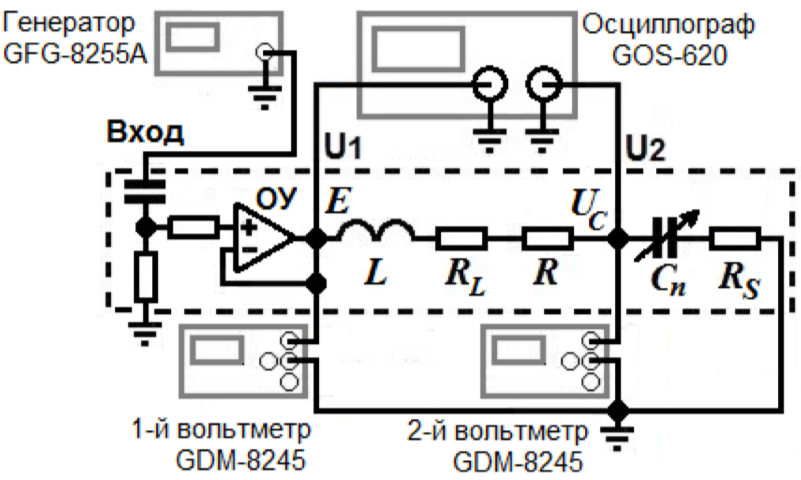
\includegraphics[width=\linewidth]{workplace.png}
        	\hspace{44pt}{Рисунок 1 -- Схема экспериментального стенда.}
        \end{wrapfigure}
        
        Схема экспериментального стенда для изучения резонанса напряжений в последовательном колебательном контуре показана на рис. 1а. Синусоидальный сигнал от генератора $GFG-8255A$ поступает через согласующую $RC-$ цепочку на вход источника напряжения, собранного на операционном усилителе ОУ. Питание операционного усилителя осуществляется встроенным блоком-выпрямителем от сети переменного тока 220 Вольт (цепь питания на схеме не показана). Источник напряжения, обладающий по определению нулевым внутренним сопротивлением, фактически обеспечивает с высокой точностью постоянство амплитуды сигнала $\mathscr{E} = \mathscr{E}_0\cos{(\omega t + \phi_0)}$ на меняющейся по величине нагрузке – последовательном колебательном контуре, изображенном на рис. 1а в виде эквивалентной схемы. Источник напряжения с согласующей цепочкой, колебательный контур и блок питания заключены в отдельный корпус с названием <<Резонанс напряжений>>, отмеченный на рисунке штриховой линией.
        
        Также имеются 7 конденсаторов, переключение между ними осуществляется вращающейся ручкой.

\newpage
\section{Теоретическая часть.}

    Будем пользоваться понятиями:
    \begin{itemize}
        \item АЧХ - амплитудно-частотная характеристика - зависимость амплитуды от частоты.
        \item ФЗЧ - фазово-частотная характеристика - зависимость сдвига фаз от частоты.
        \item Добротность - величина пропорциональная отношению запасенной в системе энергии к потерям за период, $Q = 2\pi\frac{W}{\Delta W_T}$.
        \item Колебательный контур:
            \begin{center}
                \begin{circuitikz} \draw 
                    (0,0)   to[sV,l=$\mathscr{E}_0\cos{\Omega t}$] (0,3) 
                            to[C=$C$] (3,3)
                            to[american inductor=$L$] (3,0) 
                            to[generic=$R$] (0,0);
                \end{circuitikz}
            \end{center}
        \item Векторные диаграммы:
            \begin{figure}[h!]
            	\begin{center}
            		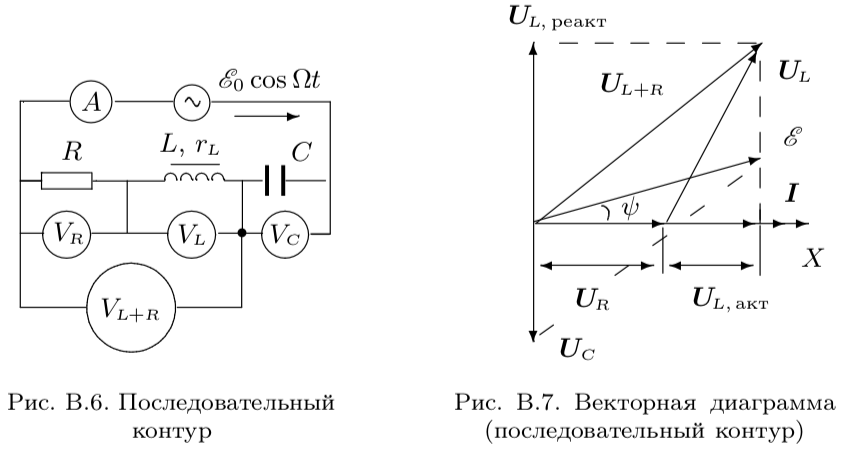
\includegraphics[width=0.8 \textwidth]{zero}\\
                	{\scriptsize
                	\begin{center}
                	\end{center}}
            	\end{center}
            \label{scheme1}
            \end{figure}
        \end{itemize}
        

\newpage
\section{Основная работа.}
    \subsection{Резонансные частоты}
        Для контуров с семью различными ёмкостями, меняя их с помощью переключателя на блоке, измерим резонансные частоты $f_{0n}$ и напряжение $U_C(f_{0n})$. Также будем регистрировать напряжение $E(f_{0n})$. Приближение к резонансу будем фиксировать при помощи фигур Лиссажу, переключая осциллограф в режим $X-Y$. Фигура Лиссажу будет представлять эллипс, оси которого направлены вдоль осей $X$ и $Y$.
        \begin{table}[!h]
            \begin{center}
           		\textbf{Таблица 1а} -- Резонансные частоты и напряжения для контуров с разными конденсаторами.\\
                \begin{tabular}{ | l | l | l | l | }
                    \hline
                    $C$, нФ &   $f_{0n}$, кГц   &  $U_c$, В & $U_E$, В  \\
                    \hline
                    24.8    &   32.423 &   0.55     &   0.0212  \\
                    33.2    &   28.023 &   0.494    &   0.0221  \\
                    47.6    &   23.423 &   0.425    &   0.0221  \\
                    57.5    &   21.337 &   0.3924   &   0.0220  \\
                    68.0    &   19.633 &   0.3644   &   0.0219  \\
                    81.6    &   17.901 &   0.3375   &   0.0218  \\
                    102.8   &   15.983 &   0.3046   &   0.0217  \\
                    \hline                
                \end{tabular}
            \end{center}
        \end{table}
        
        Сопротивление конденсатора $R = 3.5 \Omega.$
        Заполним таблицу:
        \begin{table}[!h]
            \begin{center}
           		\textbf{Таблица 1б} -- Резонансные частоты и напряжения для контуров с разными конденсаторами.\\
                \begin{tabular}{ | l | l | l | l | l | l | l | l | }
                    \hline
                    $C$, нФ    &   $L$, мкГн   &   $Q$     &  $\rho$, Ом    & $R$ сумм, Ом  & $R_{s_{max}}$, Ом   & $R_L$, Ом & $I$, мА \\
                    \hline
                    24.8    & 971.6 & 25.9  &   197.9  &    7.63    &   0.198   & 197,901 &  2.78    \\
                    33.2    & 971.6 & 22.4  &   171.1  &    7.65    &   0.171   & 171,067 &  2.89    \\
                    47.6    & 969,9 & 19.2  &   142.7  &    7.42    &   0.143   & 142,706 &  2.98    \\
                    57.5    & 967,6 & 17.8  &   129.7  &    7.27    &   0.130   & 129,766 &  3.02    \\
                    68.0    & 966,4 & 16.6  &   119.2  &    7.16    &   0.119   & 119,231 &  3.06    \\
                    81.6    & 968,7 & 15.5  &   109.0  &    7.04    &   0.109   & 109,005 &  3.10    \\
                    102.8   & 964,6 & 14.0  &   96.9   &    6.9     &   0.097   & 98,000  &  3.14    \\
                    \hline    
                    Ср.знач & 968.6 & 18.8  &   138.1  &    7.30    &   0.138   & 138     &  3.00    \\
                    \hline
                    Ср. квадратичная погр. & 0.154 & 0.242 & 2.084 & 0.017 & 0.002 & 2.07 & 0,007  \\
                    \hline
                    Стьюдента, $t_{7, 0.95}$ = 1,8946 & 18.41 & 0.49 & 3.75 & 0.14 & 0.01 & 0.5& 0,05 \\
                    \hline
                    Случайная погрешность & 1.18 & 0.056 & 0.11 & 0.02 & 0.00011 & 4.26 & 0.01 \\
                    \hline
                \end{tabular}
            \end{center}
        \end{table}
        \[
        1/\nu = 2\pi \sqrt{L/C} \text{ (условие резонанса) }, \text{ значит } L = \frac{C}{4\pi^2\nu^2}.
        \]
        \[
        Q = U_E/U_C \text{ - добротность}.
        \]
        \[
        \rho = \sqrt{L/C} \text{ - волновое (реактивное) сопротивление контура}.
        \]
        \[
        Q = \frac{\rho}{R_{\sum}}, \text{ значит } R_{\sum} = \frac{\rho}{Q}.
        \]
        \[
        R_{s_{max}} = 10^{-3}\rho.
        \]
        \[
        R_L = 2\pi\nu \cdot L.
        \]
        \[
        I = E/R_{\sum}.
        \]
        
        \begin{itemize}
            \item Точность вольтметра: 0.001 В;
            \item Точность емкости конденсатора: 0.05 нФ;
            \item Точность генератора: 0.01 кГц;
        \end{itemize}
        
        Случайная погрешность $L$:
        \[
        \sigma_L = L \cdot \sqrt{(\sigma_C/C)^2 + 2 * (\sigma_f/f)^2} = 968.6 \cdot \sqrt{(0.05/50)^2 + 2 * (0.01/20)} = 30.
        \]
        
        Случайная погрешность $Q$:
        \[
        \sigma_Q = Q \cdot \sqrt{(\sigma_{U_C}/U_C)^2 + (\sigma_{U_E}/U_E)} = 18.8 \cdot \sqrt{(0.001/0.5)^2 + (0.001/0.5)^2} = 0.056.
        \]
        
        Случайная погрешность $\rho$:
        \[
        \sigma_{\rho} = 0.5 \rho \cdot \sqrt{(\sigma_{L}/L)^2 + (\sigma_{C}/C)} = 138.1 \cdot \sqrt{(1.18/970)^2 + (0.05/50)^2} = 0.11.
        \]
        
        Случайная погрешность $R_{\sum}$:
        \[
        \sigma_{R_{\sum}} = R_{\sum} \cdot \sqrt{(\sigma_{\rho}/\rho)^2 + (\sigma_{Q}/Q)} = 7.3 \cdot \sqrt{(0.11/140)^2 + (0.056/20)^2} = 0.02.
        \]
        
        Случайная погрешность $R_{L}$:
        \[
        \sigma_{R_L} = R_L \cdot \sqrt{(\sigma_{f}/f)^2 + (\sigma_{L}/L)} = 138 \cdot \sqrt{(0.01/20)^2 + (30/970)^2} = 4.26.
        \]
        
        Случайная погрешность $I$:
        \[
        \sigma_{I} = I \cdot \sqrt{(\sigma_{U_E}/U_E)^2 + (\sigma_{R_{\sum}}/R_{\sum})} = 3 \cdot \sqrt{(0.001/0.5)^2 + (0.02/7)^2} = 0.01.
        \]
        
        Оценим вклад активных потерь в конденсаторах ($\tg\delta = 0.001$):
        \[
        R_s = \frac{1}{\omega C} \tg{\delta} = \frac{1}{2\pi 25\text{кГц}}\cdot 0.001 = 6 \cdot 10^{-9} \text{ - можно пренебречь.}
        \]
\newpage
    \subsection{Амплитудно-частотные характеристики.}
        Для контуров с двумя разными ёмкостями $C_2$ и $C_6$ снимем амплитудно-частотные характеристики (АЧХ) $U_C(f)$ для значений $U_C(f) \geq 0.6U_C(f_{0n})$ (16-17 точек в сумме по обе стороны от резонанса) при старом напряжении $E$.
        
        \begin{table}[!h]
            \begin{center}
           		\textbf{Таблица 2} -- Значения амплитуды напряжения в зависимости от частоты для $C_2$. \\
                \begin{tabular}{ | l | l | l | l | l | l | l | l | l | }
                    \hline
                    $f$, кГц & 27.237 & 27.293 & 27.644 & 27.571 & 27.441 & 27.395 & 27.793 & 27.962    \\
                    \hline
                    $U_c$, В & 0.302  & 0.313  & 0.413  & 0.391  & 0.354  & 0.340  & 0.458 & 0.487      \\
                    \hline
                    $f$, кГц & 28.268 & 28.321 & 28.381 & 28.422 & 28.386 & 28.636 & 28.552 & 28.679    \\
                    \hline
                    $U_c$, В & 0.454  & 0.439  & 0.390  & 0.410  & 0.422  & 0.345  & 0.363  & 0.324     \\
                    \hline                
                \end{tabular}
            \end{center}
        \end{table}
        \begin{table}[!h]
            \begin{center}
           		\textbf{Таблица 3} -- Значения амплитуды напряжения в зависимости от частоты для $C_6$. \\
                \begin{tabular}{ | l | l | l | l | l | l | l | l | l | }
                    \hline
                    $f$, кГц & 17.301 & 17.162 & 17.395 & 17.685 & 17.565 & 17.614 & 17.910 & 17.518    \\
                    \hline
                    $U_c$, В & 0.232  & 0.205  & 0.25   & 0.310  & 0.287  & 0.300  & 0.333 & 0.221     \\
                    \hline
                    $f$, кГц & 18.540 & 18.471 & 18.77  & 18.17  & 18.601 & 18.206 & 18.360 & 18.585    \\
                    \hline
                    $U_c$, В & 0.276  & 0.235  & 0.302  & 0.249  & 0.336  & 0.295  & 0.260  & 0.212     \\
                    \hline                
                \end{tabular}
            \end{center}
        \end{table}
        
        Построим на одном графике амплитудно-частотные характеристики в координатах $U_C(f)$, для выбранных контуров.

        \begin{center}
            \begin{tikzpicture}
                \begin{axis}[
                    title = Амплитудно-частотные характеристики для цепей с $C_2$ (справа) и $C_6$ (слева).,
                    grid = major,
                    height = 0.3\paperheight, 
        	        width = 0.8\paperwidth,
    	            xlabel = {$f$, кГц},
    	            ylabel = {$U_C$, В},
    	            xmin = 15,
    	            xmax = 30,
    	            ymin = 0.2,
    	            ymax = 0.5
                ]
                \addplot[only marks] 
                    table {
                        x       y       
                        27.237	0.302
                        27.293	0.315
                        27.643	0.413
                        27.565	0.3865
                        27.441	0.361
                        27.399	0.34
                        27.79	0.456
                        27.962	0.4874
                        28.321	0.439
                        28.322	0.4417
                        28.49	0.3978
                        28.422	0.41
                        28.636	0.345
                        28.582	0.363
                        28.679	0.324
                        28.268	0.454
                        28.1	0.487
                    };
                    \addplot[only marks] 
                    table {
                        x       y       
                        17.308	0.2311
                        17.162	0.205
                        17.395	0.25
                        17.688	0.31
                        17.566	0.286
                        17.614	0.3
                        17.907	0.333
                        18.545	0.22
                        17.522	0.28
                        18.475	0.23
                        18.183	0.3
                        18.417	0.249
                        18.006	0.331
                        18.208	0.295
                        18.361	0.261
                        18.585	0.212
                        17.796	0.328
                    };
                \end{axis}
            \end{tikzpicture}    
        \end{center}
        
        По графикам видно, что с ростом емкости конденсатора, подключенного в цепь, уменьшается амплитуда напряжения.
        
\newpage
        По данным таблиц 2 и 3 построим на одном графике амплитудно-частотные характеристики в безразмерных координатах: $x = f/f_{0n}, y = U_c(x)/U_{c1}$.
        
        \begin{center}
            \begin{tikzpicture}
                \begin{axis}[
                    title = АЧХ в безымянных координатах,
                    grid = major,
                    height = 0.25\paperheight, 
        	        width = 0.4\paperwidth,
                    xlabel = {$f/f_1$},
                    ylabel = {$U_C/U_{C_1}$},
                    xmin = 0.960,
                    xmax = 1.040,
                    ymin = 0.5,
                    ymax = 1
                ]
                \addplot[mark = o, only marks] 
                    table {
                        x       y       
                        0.972	0.612
                        0.974	0.638
                        0.986	0.837
                        0.984	0.783
                        0.979	0.731
                        0.978	0.689
                        0.992	0.924
                        0.998	0.987
                        1.011	0.889
                        1.011	0.895
                        1.017	0.806
                        1.014	0.830
                        1.022	0.699
                        1.020	0.735
                        1.023	0.656
                        1.009	0.920
                        1.003	0.986
                    };
                    \addplot[only marks] 
                    table {
                        x       y       
                        0.967	0.685
                        0.959	0.607
                        0.972	0.741
                        0.989	0.919
                        0.982	0.847
                        0.984	0.889
                        1.001	0.987
                        1.036	0.652
                        0.979	0.830
                        1.033	0.681
                        1.016	0.889
                        1.029	0.738
                        1.006	0.981
                        1.018	0.874
                        1.026	0.773
                        1.039	0.628
                        0.995	0.972
                    };
                \end{axis}
            \end{tikzpicture}    
        \end{center}
        
    Заполненные кружки соответствуют конденсатору $C_6$, пустые - $C_2$.
    
    \subsection{Фазово-частотные характеристики.}
        Для тех же двух контуров снимем фазово-частотные характеристики $\varphi_C(f)$ для значений $U_C(f) \geq 0.3U_C(f_{0n})$ (16-17 точек в сумме по обе стороны от резонанса) при старом напряжении $E$.
        
        \begin{table}[!h]
            \begin{center}
           		\textbf{Таблица 4} -- Значения фазы в зависимости от частоты для $C_2$ (слева) и $C_6$ (справа). \\
                \begin{tabular}{ | l | l | l | l | l | l | l | l | l | l |}
                    \hline
                       & $x$, см& $x_0$, см & $U_c$, В  & $f$, кГц  &    & $x$, см  & $x_0$, см & $U_c$, В  & $f$, кГц     \\
                    \hline
                    1  & 2      & 2.5       & 0.49      & 28.012    & 1  & 1.8      & 1.3       & 0.327     & 17.784  \\
                    2  & 4.2    & 3         & 0.178     & 26.429    & 2  & 3.6      & 1.9       & 0.107     & 16.264  \\
                    3  & 4.2    & 3         & 0.186     & 26.523    & 3  & 3.2      & 1.6       & 0.181     & 17.00   \\
                    4  & 4.4    & 2.8       & 0.248     & 26.985    & 4  & 2.8      & 1.4       & 0.245     & 17.367  \\
                    5  & 4.3    & 2.9       & 0.211     & 26.735    & 5  & 0.6      & 1.2       & 0.280     & 18.273  \\
                    6  & 4.6    & 2.8       & 0.282     & 27.161    & 6  & 3.4      & 1.7       & 0.148     & 16.722  \\
                    7  & 5      & 2.6       & 0.345     & 27.415    & 7  & 3        & 1.6       & 0.207     & 17.17   \\
                    8  & 3.6    & 2.6       & 0.413     & 27.640    & 8  & 2.2      & 1.4       & 0.303     & 17.640  \\
                    9  & 3.2    & 2.6       & 0.450     & 27.760    & 9  & 1        & 1.2       & 0.312     & 18.120  \\
                    10 & 0.6    & 2.4       & 0.420     & 28.400    & 10 & 0.6      & 1.2       & 0.284     & 18.260  \\
                    11 & 0.2    & 2.4       & 0.381     & 28.520    & 11 & 0.4      & 1.2       & 0.246     & 18.421  \\
                    12 & 0.2    & 2.3       & 0.315     & 28.741    & 12 & 0.2      & 1.1       & 0.221     & 18.543  \\
                    13 & 0.6    & 2.2       & 0.254     & 29.024    & 13 & 0.1      & 1         & 0.168     & 18.863  \\
                    14 & 0.8    & 2.1       & 0.199     & 29.362    & 14 & 0.1      & 0.9       & 0.126     & 19.252  \\
                    15 & 3.8    & 2.6       & 0.391     & 27.572    & 15 & 0.2      & 0.9       & 0.112     & 19.443  \\
                    16 & 4.4    & 2.7       & 0.325     & 27.340    & 16 & 0.1      & 1.1       & 0.209     & 18.665  \\
                    17 & 5      & 2.9       & 0.222     & 26.820    & 17 & 0.6      & 1.2       & 0.278     & 18.278  \\
                    \hline                
                \end{tabular}
            \end{center}
        \end{table}
        
        \begin{center}
            \begin{tikzpicture}
                \begin{axis}[
                    title = Фазово-частотные характеристики контура в зависимости от емкости конденсатора.,
                    grid = major,
                    height = 0.3\paperheight, 
        	        width = 0.8\paperwidth,
    	            xlabel = {$f/f_{0n}$},
    	            ylabel = {$\phi c/\pi$},
    	            xmin = 0.9,
    	            xmax = 1.1,
    	            ymin = -0.1,
    	            ymax = 2.1
                ]
                \addplot[mark = o, only marks] 
                    table {
                        x       y       
                        1.000	0.800   
                        0.943	1.400
                        0.946	1.400
                        0.963	1.571
                        0.954	1.483
                        0.969	1.643
                        0.978	1.923
                        0.986	1.385
                        0.990	1.231
                        1.013	0.250
                        1.018	0.083
                        1.026	0.087
                        1.036	0.273
                        1.048	0.381
                        0.984	1.462
                        0.976	1.630
                        0.957	1.724
                    };
                    \addplot[only marks] 
                    table {
                        x       y       
                        0.994	1.385
                        0.901	1.895
                        0.950	2.000
                        0.970	2.000
                        1.021	0.500
                        0.935	2.000
                        0.959	1.875
                        0.986	1.571
                        1.013	0.833
                        1.020	0.500
                        1.029	0.333
                        1.036	0.182
                        1.054	0.100
                        1.076	0.111
                        1.086	0.222
                        1.040	0.091
                        1.022	0.500
                    };
                \end{axis}
            \end{tikzpicture}    
        \end{center}
    
    Заполненные кружки соответствуют конденсатору $C_6$, пустые - $C_2$.
    
    \subsection{Добротность.}
        Найдем добротность $Q$, используя амплитудно-частотные и фазово-частотные характеристики.
        
        \begin{itemize}
            \item По ширине резонансных кривых на уровне $0.707$ определим добротности $Q$ соответствующих контуров: 
            
            $Q = \omega_0 / 2\Delta \Omega$
            \begin{itemize}
                \item $Q_{C_2}$ = 21;
                \item $Q_{C_6}$ = 18.
            \end{itemize}
            
            Более острая совокупность точек соответствует $C_2$, более широкая - $C_6$. Чем пик острее тем добротность больше.
            
            Оценим погрешность:
            \[
            \sigma_Q = 0.1
            \]
            \[
            \epsilon_{Q_{C_2}} = 0.5/21 = 0.024 = 2.4\%
            \]
            \[
            \epsilon_{Q_{C_6}} = 0.5/18 = 0.027 = 2.7\%
            \]        
            Итого:
            \[
            Q_{C_2} = 21 \pm 0.1, \epsilon_{Q_{C_2}} = 2.4\%
            \]
            \[
            Q_{C_6} = 18 \pm 0.1, \epsilon_{Q_{C_6}} = 2.7\%
            \]
\newpage
            \item По расстоянию между точками по оси $x$, в которых $y$ меняется от $-1/4$ до $1/4$. Это расстояние равно $1/Q$.
            \begin{itemize}
                \item $x_1$ = 0.04
                \item $x_2$ = 0.06
            \end{itemize}
            Более быстрорастущая совокупность точек соответствует $C_2$, более широкая - $C_6$. Чем рост быстрее тем добротность больше.
            \[
            1/Q_{C_2} = x_1 = 0.04
            \]
            \[
            1/Q_{C_6} = x_2 = 0.06
            \]
            \[
            Q_{C_2} = 20 
            \]
            \[
            Q_{C_6} = 16.6 
            \]
            Оценим погрешность:
            \[
            \sigma_x = 0.01
            \]            
            \[
            \sigma_{Q_{C_2}} = Q_{C_2} \cdot 0.01/0.04 = 20 \cdot 0.25 = 5
            \]
            \[
            \sigma_{Q_{C_6}} = Q_{C_6} \cdot 0.01/0.06 = 16.6 \cdot 0.16 = 2.8
            \]
             Итого:
            \[
            Q_{C_2} = 20 \pm 5, \epsilon_{Q_{C_2}} = 25\%
            \]
            \[
            Q_{C_6} = 16.6 \pm 2.8, \epsilon_{Q_{C_6}} = 16.7\%
            \]
            \end{itemize}
        
    \subsection{Зависимость $R_L(f_{0n})$.}
        По данным таблиц 1 и 2 построим зависимость $R_L(f_{0n})$.
        \begin{center}
            \begin{tikzpicture}
                \begin{axis}[
                    title = Зависимость $R_L(f_{0n})$,
                    grid = major,
                    height = 0.3\paperheight, 
        	        width = 0.8\paperwidth,
    	            xlabel = {$f_{0n}$, кГц},
    	            ylabel = {$R_L$, Ом},
    	            xmin = 8.5,
    	            xmax = 20.5,
    	            ymin = 85,
    	            ymax = 205,
    	            legend pos = north west,
                ]
                \legend{ 
    	            ,$y = -10.109x + 0.873$
                };
                \addplot[only marks] 
                    table {
                        x       y       
                        19.4568	197.901
                        16.8138	171.067
                        14.058	142.706
                        12.798	129.766
                        11.778	119.231
                        10.7358	109.005
                        9.4788	98.000
                    };
                \addplot[dashed, draw = blue] coordinates {
                        (9,91.854) (20,203.05)
                    };
                \end{axis}
            \end{tikzpicture}    
        \end{center}
        
    Возможной причиной роста сопротивления с увеличением частоты могут быть возникающие в катушке паразитные токи, на которые тратится энергия.
    
    \subsection{Вывод.}
        В работе исследовали резонанс напряжений в последовательном контуре. Нашли резонансную частоту при помощи фигур Лиссажу. Определили добротность колебательного контура тремя способами. Обнаружили зависимость между сопротивлением катушки, добротностью и частотой на примере двух конденсаторов.
\end{document}
